\documentclass{beamer}
\graphicspath{{../report/figures/}}
\usepackage{listings}
\usepackage{ulem}
\usepackage{subcaption}
\captionsetup{compatibility=false}
\usepackage[linesnumbered]{algorithm2e}
\usepackage{multicol}
%\usepackage[danish]{babel}
\usepackage[T1]{fontenc}
\usepackage[utf8]{inputenc}
\usepackage{multirow}

\newcommand{\linespace}{\vspace{1em}}

\mode<presentation>
{
  \usetheme{Darmstadt}
  \setbeamertemplate{footline}[frame number]
  \setbeamertemplate{navigation symbols}{}
  \setbeamercovered{transparent}
}

\AtBeginSection[]
{
   \begin{frame}
        \frametitle{Overview}
        \tableofcontents[sectionstyle=show/hide,subsectionstyle=show/show/hide]
   \end{frame}
}

\title[The Launcher for the GIRAF Software Suite]{The Launcher for the GIRAF Software Suite}
\subtitle{SW605F14}
\author[SW605F14]{Jesper Byrdal Kj\ae r, Frederik Bruhn Mikkelsen, \\Stefan Mailund Thilemann, Anders Vagner}
\institute[Aalborg University]
{
  Department of Computer Science\\
  Aalborg University}

\date[CFP 2003]{June 19th, 2014}

\begin{document}

%--------------------------------------------------
%     SLIDES
%--------------------------------------------------
\begin{frame}
  \titlepage
\end{frame}

\begin{frame}
    \frametitle{Content}
    \tableofcontents[sectionstyle=show/show,subsectionstyle=hide/hide/hide]
\end{frame}

\section{Introduction}
\subsection{Multi-project}
\begin{frame}{Management of the multi-project}
	The multi-project consists of
	\begin{description}
		\item[Students:]{60}
		\item[Groups:]{16}
	\end{description}

	Development method: Scrum
	\begin{description}
		\item[Sprints]{Project split into four sprints}
		\begin{itemize}
			\item[Sprint 1] 24-02-2014 -- 19-03-2104 
			\item[Sprint 2] 20-03-2014 -- 14-04-2104
			\item[Sprint 3] 15-04-2014 -- 07-05-2104
			\item[Sprint 4] 08-05-2014 -- 27-05-2104
		\end{itemize}
	\end{description}
\end{frame}

\begin{frame}{Roles and responsibilities}
	Roles assigned on multi-project level and their responsibilities
	\begin{description}
		\item[Scrum Master] Chairing Scrum meetings and coordination of groups and meetings.
		\item[Sprint End Specialist] Coordinator and chairman of sprint review meetings.
		\item[Client Contact] Responsible for all communication to and from the clients.
	\end{description}
\end{frame}

\subsection{Structure}
\begin{frame}{Structure of the multi-project}
\begin{columns}
\begin{column}{.38\textwidth}
\begin{itemize}
\item Using scrum on 16 groups requires Scrum of Scrums
\item One meeting each week, for all groups
\end{itemize}
\end{column}
\begin{column}{.58\textwidth}
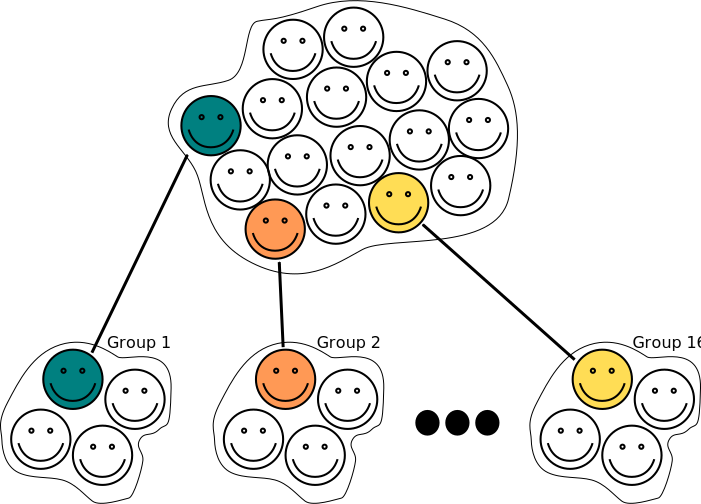
\includegraphics[width=\textwidth]{pres/scrumofscrums}
\end{column}
\end{columns}
\end{frame}

\subsection{Graphical Interface Resources for Autistic Folk (GIRAF)}
\begin{frame}{Project overview}
	\begin{itemize}
		\item<1> The purpose of GIRAF
		\item<2> Collection of front-end and back-end applications
		\item<3> The goals of the semester for GIRAF
		\begin{center}
		\includegraphics<2>[width=0.8\textheight]{pres/girafstructure}
		\end{center}
	\end{itemize}
\end{frame}

\subsection{The Launcher Project}
\begin{frame}{Launcher}
	\begin{description}
		\item<1>[What is Launcher]{An application launcher}
		\includegraphics<1>[width=0.8\textheight]{pres/launcherdescription}
		\item<2>[Permissions] Restriction of access to the android system
		\item<3>[Users] Management of users
	\end{description}
\end{frame}

\begin{frame}{Structure}
	\center
	\begin{center}
		\includegraphics[width=\textwidth]{pres/launcherstructure}	
	\end{center}
\end{frame}

\section{Project Overview}
\subsection{Project Summary}
\begin{frame}
\frametitle{Sprint One}
\textbf{Main purpose:}\\
\only<1>{Bug fixing \qquad\includegraphics[height=4cm]{images/bugfixing}}
\only<2>{Improve Drawer \quad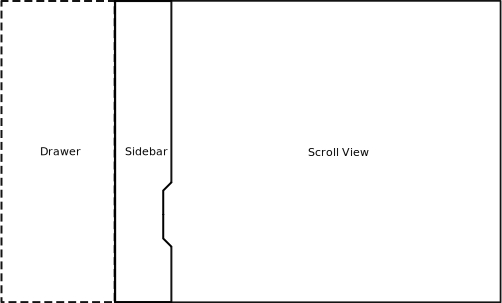
\includegraphics[height=4cm]{images/drawer}}
\only<3>{Carry out functional tests \quad\includegraphics[height=4cm]{images/test}}
\end{frame}

\begin{frame}
\frametitle{Sprint One}
\begin{center}
Demonstration
\end{center}

\end{frame}

\begin{frame}
\frametitle{Sprint Two}
\textbf{Main purpose:}\\
\only<1>{Create Prototypes of Settings \quad\includegraphics[height=4cm]{images/prototype}}
\only<2>{Receive feedback from customer meetings \quad\includegraphics[height=4cm]{images/customer}}

\end{frame}

\begin{frame}
\frametitle{Sprint Three}
\textbf{Main purpose:}
\pause
\begin{itemize}
\item Start implementation of Settings
\begin{itemize}
\pause
\item Settings for Launcher
\pause
\item Application Management
\pause
\item Settings for Cars and Sequence
\end{itemize}
\end{itemize}
\end{frame}

\begin{frame}
\frametitle{Sprint Four}
\textbf{Main purpose:}
\pause
\begin{itemize}
\item Finish implementation of Settings
\pause
\end{itemize}

\begin{center}
Demonstation
\end{center}
\end{frame}

\section{Collaboration}
\subsection{Sprint End Organisation}

\begin{frame}{The First Sprint Review}
	This meeting had some fundamental problems:
	\begin{itemize}
		\item No feedback from the clients.
		\item Technical problems with the demonstrations.
		\item Obscure presentations.
		\item Only a few clients were able to attend.
	\end{itemize}
	So, a Sprint End specialist was appointed.
\end{frame}

\begin{frame}{Sprint End Collaboration}
	As the specialist was in this group, we had several tasks in connection with the sprint reviews:
	\begin{itemize}
		\item Instructing the groups on how to present their progress.
		\item Testing that all applications worked together.
		\item Helping groups with last-minute integration problems.
		\item Conduct the client install party.
		\item Host the sprint review meeting.
	\end{itemize}
\end{frame}


\subsection{The Remote Database}

\begin{frame}{Integrating the Remote Database}
	LocalDB had become a component in \textit{Launcher}.\\
	\vspace{\baselineskip}
	Near the end of the fourth sprint, the remote database group were ready to activate synchronisation.\\
	\vspace{\baselineskip}
	We chose to go ahead with this.
\end{frame}

\begin{frame}{Integration Problems}
	The attempt to implement this resulted in several problems:
	\begin{itemize}
		\item Inconsistencies between the two databases.
		\item Inconsistencies between the applications and the modified local database.
		\item The inability of \textit{Pictoseach} to handle large numbers of pictograms.
	\end{itemize}

	\begin{block}{Frederic P. Brooks (1995)}
    	\textit{``All programmers are optimists.''}
   	\end{block}
\end{frame}


\subsection{Multi-Project Management}

\begin{frame}{Roles}
	Roles we used:
	\begin{itemize}
		\item Scrum Master
		\item Client Contact
		\item Sprint End Specialist
	\end{itemize}
	Missing:
	\begin{itemize}
		\item Product Owner
	\end{itemize}
\end{frame}

\begin{frame}{Use of Scrum}
	Scrum only worked to a limited degree.\\
	\vspace{\baselineskip}
	It has been suggested to recommend another method (e.g. UP) to future teams.\\
	\vspace{\baselineskip}
	We however would recommend studying the chosen method extensively, and then implement it right.
\end{frame}



\section{Evaluation}
%---------------------%
%     Use of Scrum     %
%-------------------- %
\subsection{Use of Scrum}
\begin{frame}{Development Method}
  What is Scrum?
  \begin{itemize}
  \item Framework used to address complex adaptive problems
    \begin{itemize}
    \item Ensures products of highest possible value
    \end{itemize}
  \end{itemize}

	\begin{figure}
		\includegraphics[width=1\textwidth]{slides/agile-glossary.png}
	%	\caption{http://www.scrumhint.com/wp-content/uploads/2013/05/agile-glossary.png}
	\end{figure}
\end{frame}

\begin{frame}{Multi-Project Scrum usage}
  \begin{columns}
  		\begin{column}{0.5\textwidth}
  			Decision based on:
  			\begin{itemize}
      		\item Recommended by Semester Coordinator
        		\begin{itemize}
        		\item Familar to all students
        		\end{itemize}
      		\item Sprint length
        		\begin{itemize}
        		\item Fits study project well
        		\end{itemize}
      		\item Supported by tools
        \end{itemize}
  		\end{column}
  		
  		\pause
  		
  		\begin{column}{0.5\textwidth}
        Roles utilized:	
  	    \begin{itemize}
      	  \item Scrum Roles
        	  \begin{itemize}
        	    \item Scrum Master
        	  \end{itemize}
      		\item Ad-hoc Scrum Roles
        		\begin{itemize}
  	      		\item Client Contact
  	      		\item Sprint End Specialist
        		\end{itemize}
      	\end{itemize}
      	\pause
  	    \linespace
  			Missing essential parts:
    				\begin{itemize}
    				\item Product Owner
    				\pause
    				\item \textit{Scrum Master?}
    				\end{itemize}
  		\end{column}
  \end{columns}
\end{frame}

\begin{frame}{Group Scrum usage}
	Intentions to use Scrum in group, to:
	\begin{itemize}
		\item Synchronize progress with multi-project Scrum
	\end{itemize}
	\begin{center}
	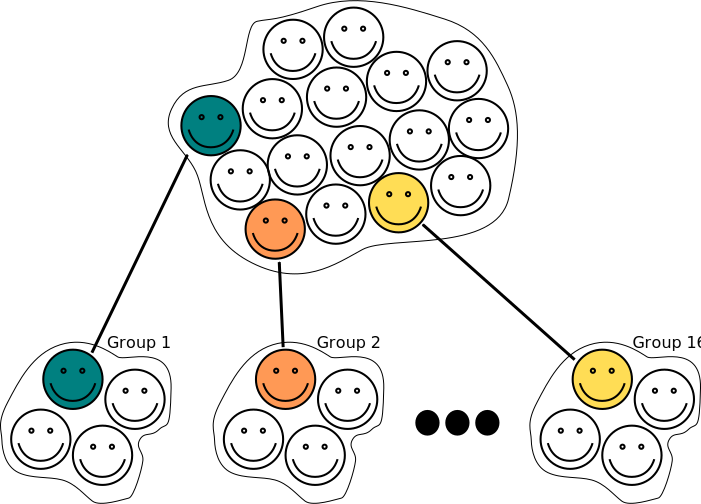
\includegraphics[width=0.6\textwidth]{pres/scrumofscrums}
	\end{center}
\end{frame}

\begin{frame}{Group Scrum usage}
  Did not work as expected:
  \pause
  \begin{itemize}
    	\item Failed to sustain Scrum Events
    			\begin{itemize}
    			\item Sprint Planning
    			\item Daily Scrum
    			\item Sprint Review
    			\end{itemize}
    			\pause
    \item Did not utilize Scrum Roles
  \end{itemize}
\end{frame}

\begin{frame}{Conclusion on using Scrum}
  \begin{block}{Official Scrum Guide says:}
  \textit{''Scrum’s roles, artifacts, events, and rules are immutable and although implementing only parts of Scrum is possible, the result is not Scrum. 
  Scrum exists only in its entirety and functions well as a container for other techniques, methodologies, and practices.''}
  \end{block}
\end{frame}

\begin{frame}{Conclusion on using Scrum}
  Even though Scrum was not utilized properly, the following was achieved by using Scrum both for the multi-project, but also for the Launcher project:
  \pause
  \begin{itemize}
    \item Providing structure
    \pause
    \item Distribution of responsibilities
    \pause
    \item Driving development towards common goal and maintaining clients interests
  \end{itemize}
  \pause
  \linespace
  \begin{block}{Recommandation for next GIRAF developers}
  Investigate multiple methodologies thoroughly, before starting any developments.
  Commit to the chosen methodology!
  \end{block}
\end{frame}

%--------------------------------------------------
%     OOD
%--------------------------------------------------
\subsection{System Design}
\begin{frame}{Developments}
	\begin{itemize}
		\item<1> Taking over an existing project
  		\begin{itemize}
    		\item Refactoring vs. Rewriting
  		\end{itemize}
		\item<2> ``Ad-hoc'' design
  		\begin{itemize}
  		\item Case: View Holder pattern, Android best-practice
  		\end{itemize}
		\begin{center}
		\includegraphics<1,2>[width=0.8\textheight]{slides/swengineer}
		\end{center}
	\end{itemize}
\end{frame}

\begin{frame}{Design Patterns}
  \begin{itemize}
  \item<1> Identify possible patterns to use
  \item<2> Suggestion: Observer Pattern
    \begin{itemize}
    \item Loading of application into View
    \end{itemize}
  \end{itemize}
  
  \includegraphics<2>[width=1\textwidth]{slides/observer.png}
\end{frame}





\section{Summary}
\subsection{Future works}
\begin{frame}{Backlog}
	
	\begin{block}{Features requested but not implemented}
	\begin{description}
		\item[Copy settings]{}
		\end{description}
	\vspace{-0.5em}
		It should be possible to copy settings from one user to another.
	\end{block}
	\vspace{\baselineskip}
	
	\begin{block}{Improvements}
	\begin{description}
		\item[Downloading data]{}
	\end{description}
	\vspace{-0.5em}
	Pictograms should be downloaded while tablet is being used.
	\vspace{1em}
	\begin{description}
		\item[Loading applications]{}
	\end{description}
	\vspace{-0.5em}
	The process of showing applications in the activities needs refactoring.
	\end{block}
\end{frame}

\subsection{Conclusion}
\begin{frame}{Conclusion}
\begin{block}{Project Goals}
	\begin{itemize}
		\item Running applications
		\item Fulfill client requirements
	\end{itemize}
\end{block}
\vspace{1em}
\pause
	The Launcher works, but the things left in the backlog still need to be addressed.\\
	Furthermore, the Launcher must adjust to the changes done to the other applications.
\end{frame}


\end{document}